\chapter{Petalinux project: from start to bottom}
Now that all the tools and utilities are installed and the environment is ready, it is possible to create the first petalinux project. The environment created on the server is the one shown in Figure \ref{fig:server}
\begin{figure}[ht]
	\centering
	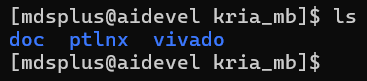
\includegraphics[width=0.5\textwidth]{images/server}
	\caption{Environment set-up.}
	\label{fig:server}
\end{figure}
in which  the folder \textit{doc} is used to store all the documents needed for the project creation, the folder \textit{vivado} will contain all the Vivado prject and the folder \textit{ptlnx} is the installation folder of petalinux-v2022.2.

A prerequisite is having already generated the bitstream and exported the hardware description from the Vivado project.

\subsection{Building the project}
From the AMD download page, download the .BSP file of the board it is about to be used. Inside petalinux installation folder, create another folder named prj. (here all the projects will be created, build and saved) and copy the .BSP file in this directory. Move now into this folder. As the first task, upgrade petalinux eSDK typing (everything on the sane line)
\begin{verbatim}
	petalinux-upgrade -u http://petalinux.xilinx.com/sswreleases/rel-v2022
	/sdkupdate/2022.2_update1/ -p "aarch64" --wget-args "--wait 1 -nH --cut-dirs=4"
\end{verbatim}
To create the project, type
\begin{verbatim}
	petalinux-create --type project -s <BPS_FILE_PATH> --name <PROJECT_NAME>
\end{verbatim}
and move into the created folder. The next step is to configure the project with the following command line (the HARDWARE\_FILE\_PATH is the file with the extension .xsa in the Vivado project folder)
\begin{verbatim}
	petalinux-config --get-hw-description <HARDWARE_FILE_PATH>
\end{verbatim}
after which a window like the one of Figure \ref{fig:prj3}.
\begin{figure}[ht]
	\centering
	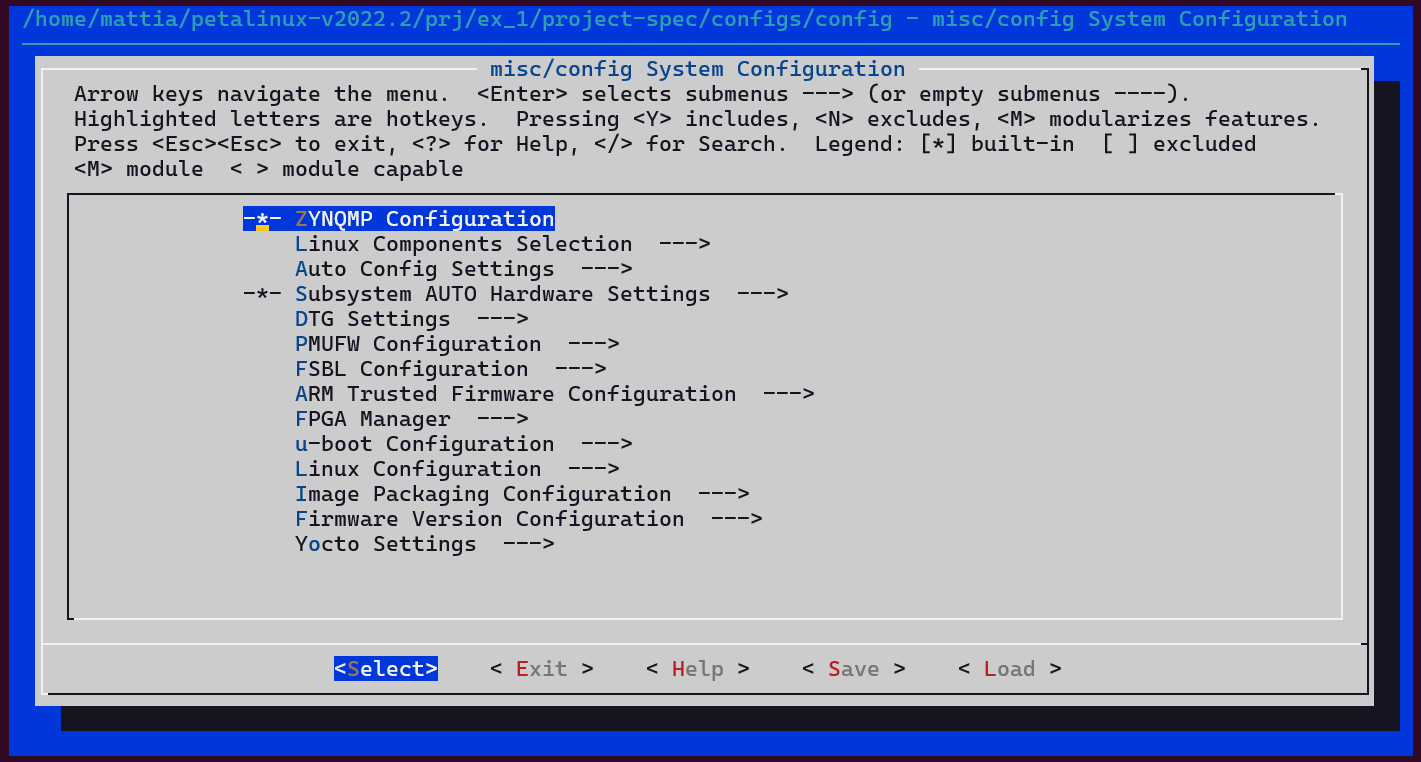
\includegraphics[width=0.65\textwidth]{images/prj3}
	\caption{Petalinux configuration window.}
	\label{fig:prj3}
\end{figure}
Following the instructions, navigate into the folders below reported and change the respective configurations:
\begin{itemize}
	\item \textit{FPGA Manager $-->$ Fpga Manager[*]}
	\item \textit{Image Packaging Configuration $-->$ Root Filesystem Type --> INITRD[*]}
	\item \textit{Image Packaging Configuration $-->$ INITRAMFS/INITRD Image name $-->$ petalinux-initramfs-image}
	\item \textit{Image Packaging Configuration $-->$ Copy final images to tftpboot[]}
\end{itemize}
Exit and save the project. It is possible now to build the project. Type
\begin{verbatim}
	petalinux-build
\end{verbatim}
and let the machine to run. After this operation, it is possible to add, if needed, various kernel packages typing
\begin{verbatim}
	petalinux-config -c kernel
\end{verbatim}
The next step is to configure the root file system (see Figure \ref{fig:prj7}) with the command
\begin{verbatim}
	petalinux-config -c rootfs
\end{verbatim}
from which all the needed packages are installed. An example fo the packages installed ca be (acceleration, XRT and gcc):
\begin{itemize}
	\item Filesystem Packages $-->$ console $-->$ utils $-->$ git $-->$ [*] git
	\item Filesystem Packages $-->$ base $-->$ dnf $-->$ [*] dnf
	\item Filesystem Packages $-->$ x11 $-->$ base $-->$ libdrm $-->$ [*] libdrm
	\item Filesystem Packages $-->$ x11 $-->$ base $-->$ libdrm $-->$ [*] libdrm-tests
	\item Filesystem Packages $-->$ x11 $-->$ base $-->$ libdrm $-->$ [*] libdrm-kms
	\item Filesystem Packages $-->$ libs $-->$ xrt $-->$ [*] xrt
	\item Filesystem Packages $-->$ libs $-->$ xrt $-->$ [*] xrt-dev
	\item Filesystem Packages $-->$ libs $-->$ zocl $-->$ [*] zocl 
	\item Filesystem Packages $-->$ libs $-->$ opencl-headers $-->$ [*] opencl-headers 
	\item Filesystem Packages $-->$ libs $-->$ opencl-clhpp $-->$ [*] opencl-clhpp-dev
	\item Filesystem Packages $-->$ misc $-->$ packagegroup-core-buildessential $-->$ packagegroup-core-buildessential[*]
	\item Filesystem Packages $-->$ misc $-->$ packagegroup-core-buildessential $-->$ packagegroup-core-buildessential[*]
	\item Filesystem Packages $-->$ misc $-->$ gcc-runtime $-->$ libstdc++[*]
	\item Petaliunx Package Groups $-->$ packagegroup-petalinux $-->$ [*] packagegroup-petalinux
	\item Petaliunx Package Groups $-->$ packagegroup-petalinux-gstreamer $-->$ [*] packagegroup-petalinux-gstreamer
	\item Petaliunx Package Groups $-->$ packagegroup-petalinux-opencv $-->$ [*] packagegroup-petalinux-gstreamer
	\item Petaliunx Package Groups $-->$ packagegroup-petalinux-v4lutils $-->$ [*] packagegroup-petalinux-gstreamer
	\item Petaliunx Package Groups $-->$ packagegroup-petalinux-x11 $-->$ [*] packagegroup-petalinux-gstreamer
\end{itemize}
\begin{figure}[ht]
	\centering
	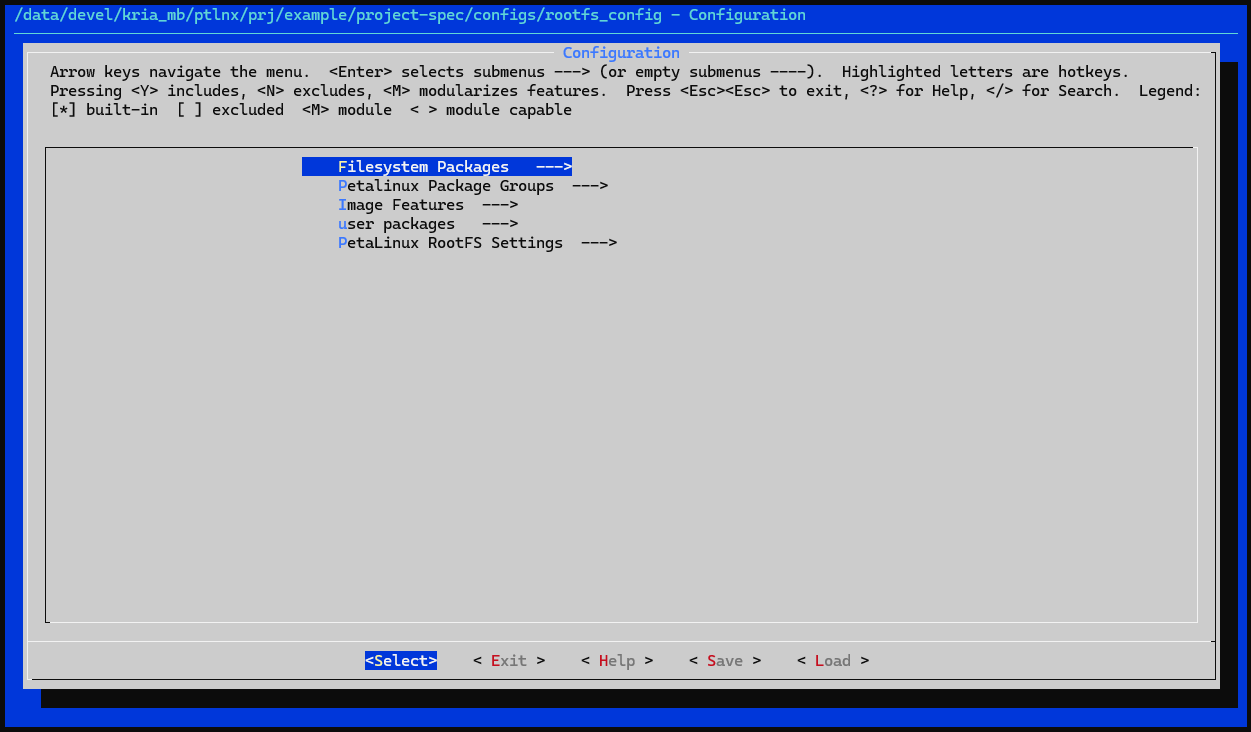
\includegraphics[width=0.65\textwidth]{images/prj7}
	\caption{Petalinux root configuration window.}
	\label{fig:prj7}
\end{figure}
After exiting the window, rebuild the project. The last step in order to finish the project creation is to build the SDK with the command
\begin{verbatim}
	petalinux-build --sdk
\end{verbatim}

\subsection{Preparing the SD-card}
There are two possible ways to prepare the SD-card for the KRIA KR260: create the .wic file to be flashed directly into the SD or to create the partitions on the SD-card and upload the needed files in the respective partitions. The first step is, anyway, to generate the images
\begin{verbatim}
	petalinux-package --boot --u-boot --force
\end{verbatim}


\subsubsection{.wic file creation}
To generate the .wic file. type into the command line (on the same line)
\begin{verbatim}
	petalinux-package --wic --images-dir images/linux/ --bootfiles
	"ramdisk.cpio.gz.u-boot,boot.scr,Image,system.dtb,system-zynqmp-sck-kr-g-revB.dtb"
	--disk-name "sda"
\end{verbatim}
and let the machine to create the file. After that it is possible to flash it to the SD-card with Balena Etcher (or another program just alike).


\subsubsection{SD-card partitioning}
Another possible, but a bit more complex, way to boot the KR260 from SD is to partition the SD card and move into the apposite partitions the needed images. To fully understand this method, please refer to \href{https://xilinx-wiki.atlassian.net/wiki/x/EYMfAQ}{this} page. 

\textbf{Warning}: approaching this method from WSL is not possible. There are some problems between the interface of the SD cards / USB connectors and the virtual machine.

\subsection{Booting the board}
To boot the board it is simply needed to insert the SD-card into the apposite slot, connect the power and the USB cable to a computer. To read the data stream, download a terminal application like PuTTY. After the boot, it is necessary to log in the system. It will request a username and a password:
\begin{verbatim}
	username: petalinux
	passowrd: your_password
\end{verbatim}
\begin{figure}[ht]
	\centering
	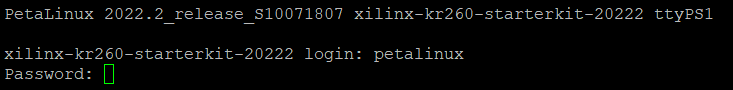
\includegraphics[width=0.65\textwidth]{images/boot1}
	\caption{Booting board.}
	\label{fig:boot1}
\end{figure}